\chapter{插值 POD 方法的应用实例与数据对比分析}
\label{cha:usage-example}

\section{单变量POD插值算例}
\label{sec:single_variable_pod}
考虑单一参数扰动情形(如混合角$\lambda_\alpha$),设采样点集为$\{\lambda_{\alpha}^{(k)}\}_{k=1}^m$,对应POD基矩阵$\{\Phi^{(k)}\}_{k=1}^m$。对任意新参数$\lambda_\alpha^*$,基于三次样条的插值基矩阵可表示为分段多项式组合:

\begin{equation}
    \Phi^* = \sum_{k=1}^m S_k(\lambda_\alpha^*) \Phi^{(k)}
    \label{eq:single_spline}
\end{equation}

式中$S_k(\lambda_\alpha)$为三次样条基函数,满足$C^2$连续条件。

基于公式\eqref{eq:single_spline}的插值POD方法,选取NACA0012翼型在$M=0.8$条件下进行验证。设置迎角扰动变量$\alpha\in[-1.25^\circ,1.25^\circ]$,采样间隔$\Delta\alpha=0.25^\circ$,共获取11组训练样本。图\ref{fig:cp_samples}展示了采样工况的压力系数分布,图\ref{fig:interp_validation}则重点呈现插值方法在非采样工况($\alpha=0.45^\circ,0.77^\circ$)的预测性能。

\begin{figure}[H]
\centering
\captionsetup[subfigure]{font=scriptsize} % 子图字号
\begin{subfigure}[b]{0.18\textwidth}
\centering
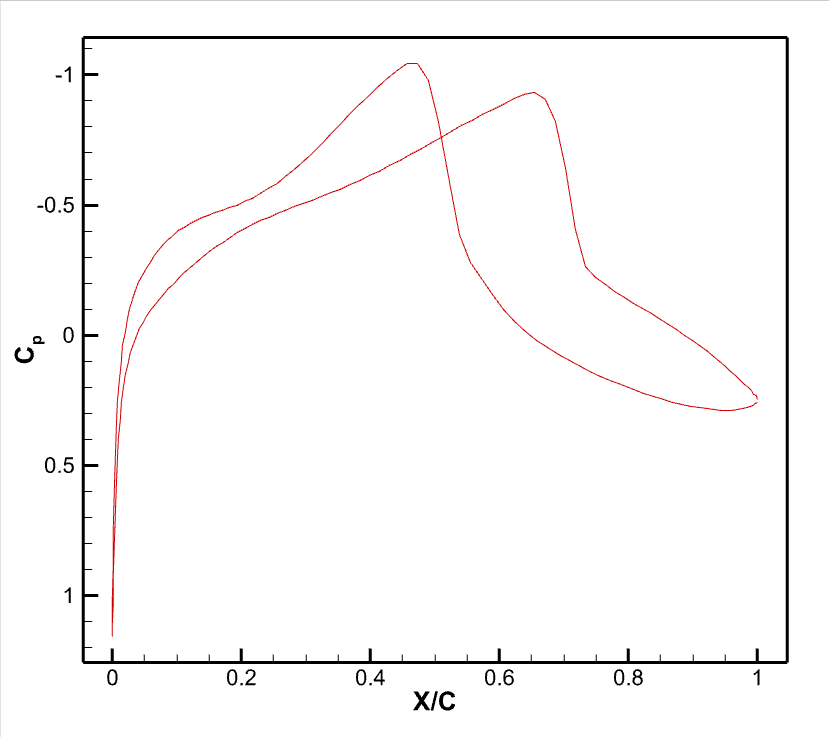
\includegraphics[width=\linewidth]{1.png}
\caption{$\alpha=-1.25^\circ$}
\end{subfigure}
\hfill
\begin{subfigure}[b]{0.18\textwidth}
\centering
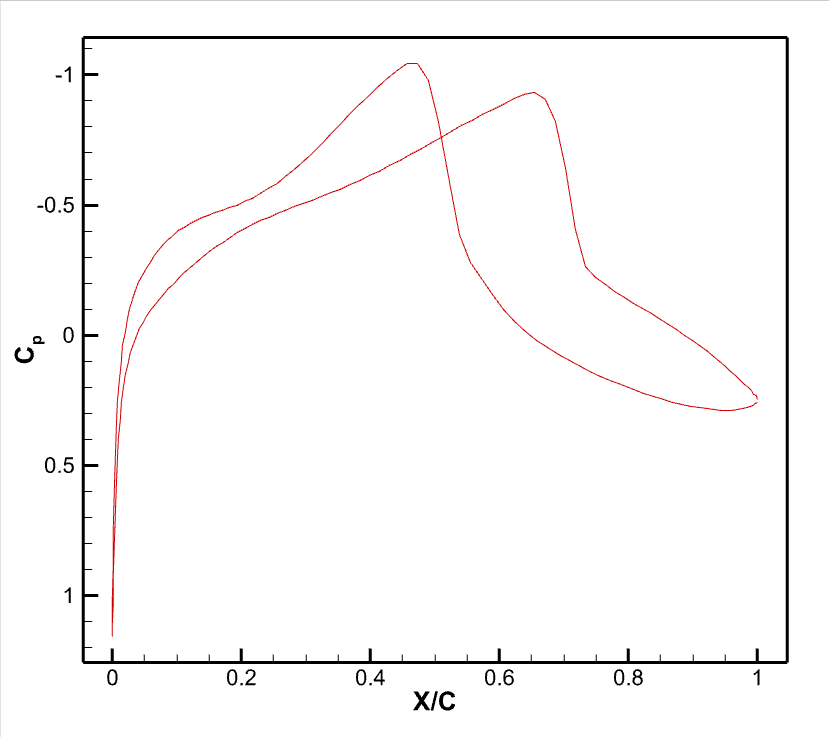
\includegraphics[width=\linewidth]{2.png}
\caption{$\alpha=-1.00^\circ$}
\end{subfigure}
\hfill
\begin{subfigure}[b]{0.18\textwidth}
\centering
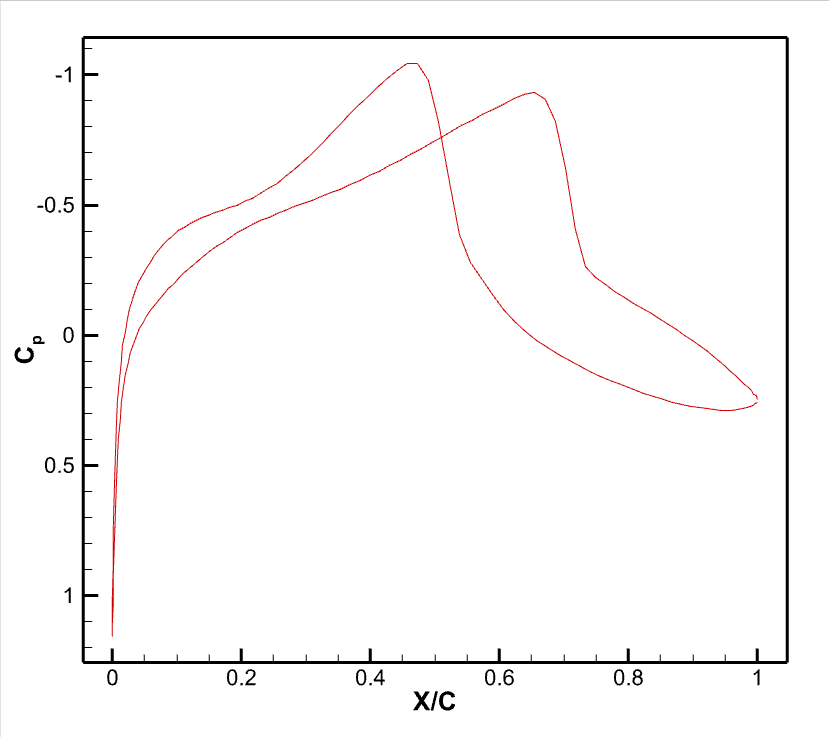
\includegraphics[width=\linewidth]{3.png}
\caption{$\alpha=-0.75^\circ$}
\end{subfigure}
\hfill
\begin{subfigure}[b]{0.18\textwidth}
\centering
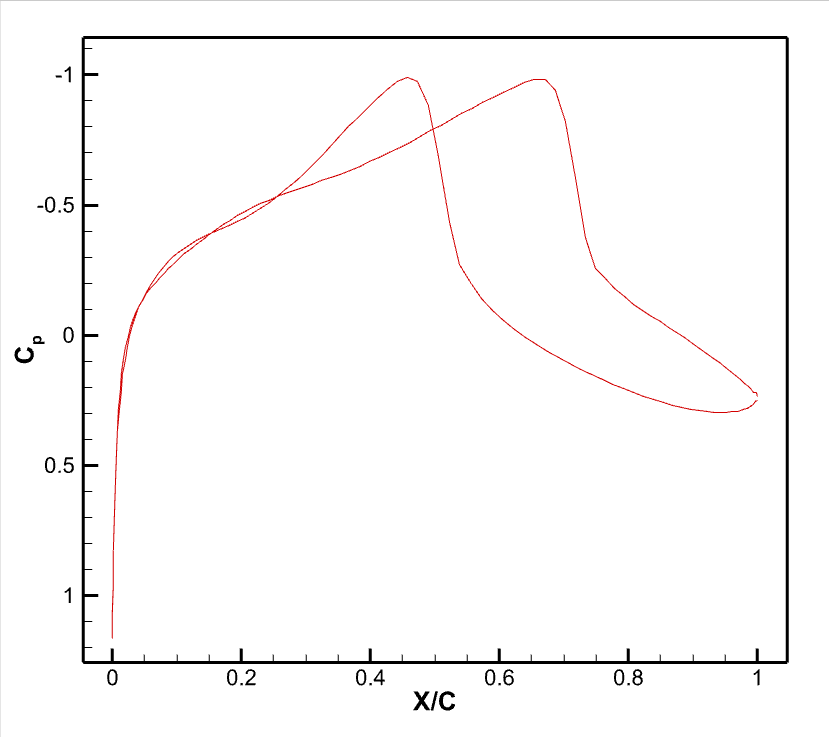
\includegraphics[width=\linewidth]{4.png}
\caption{$\alpha=-0.50^\circ$}
\end{subfigure}
\hfill
\begin{subfigure}[b]{0.18\textwidth}
\centering
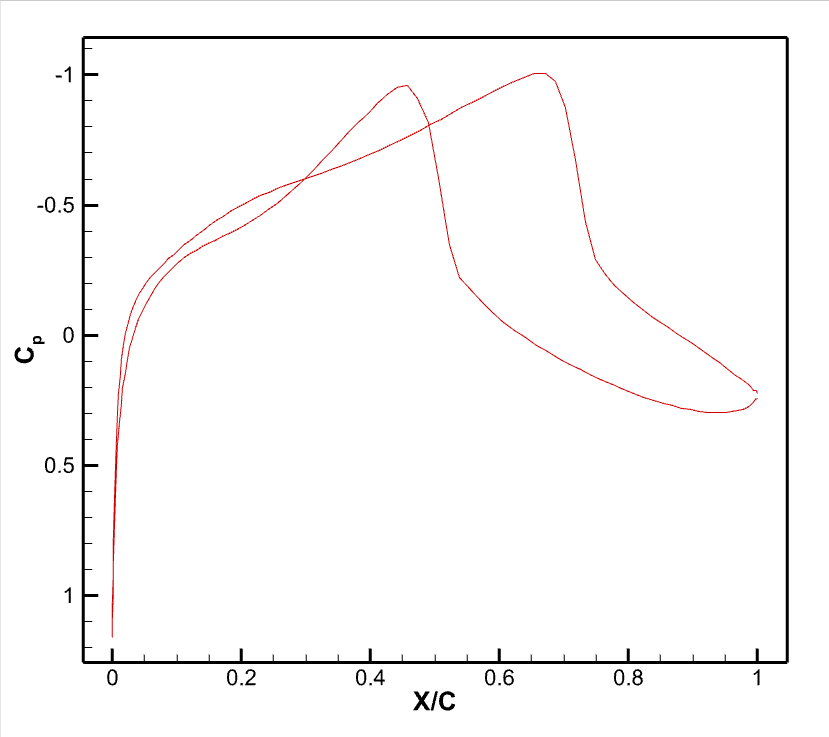
\includegraphics[width=\linewidth]{5.png}
\caption{$\alpha=-0.25^\circ$}
\end{subfigure}

\vspace{0.5cm} % 行间距

\begin{subfigure}[b]{0.18\textwidth}
\centering
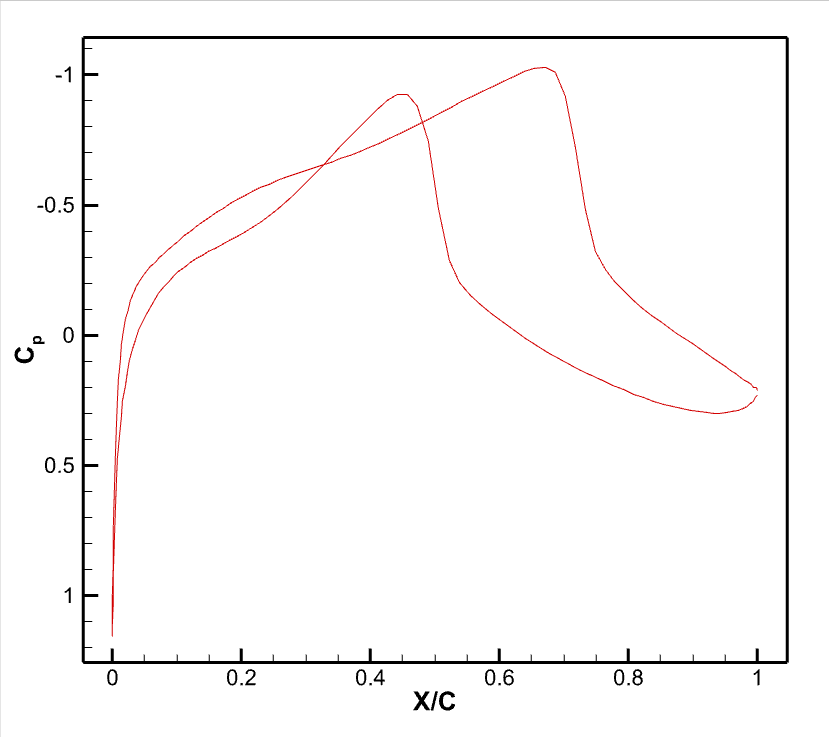
\includegraphics[width=\linewidth]{6.png}
\caption{$\alpha=0.00^\circ$}
\end{subfigure}
\hfill
\begin{subfigure}[b]{0.18\textwidth}
\centering
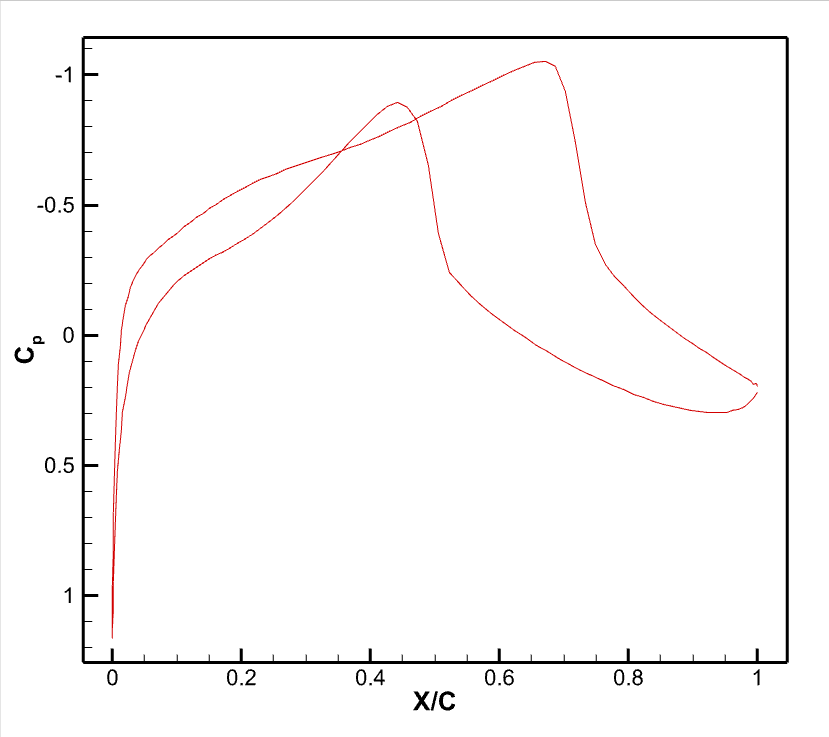
\includegraphics[width=\linewidth]{7.png}
\caption{$\alpha=0.25^\circ$}
\end{subfigure}
\hfill
\begin{subfigure}[b]{0.18\textwidth}
\centering
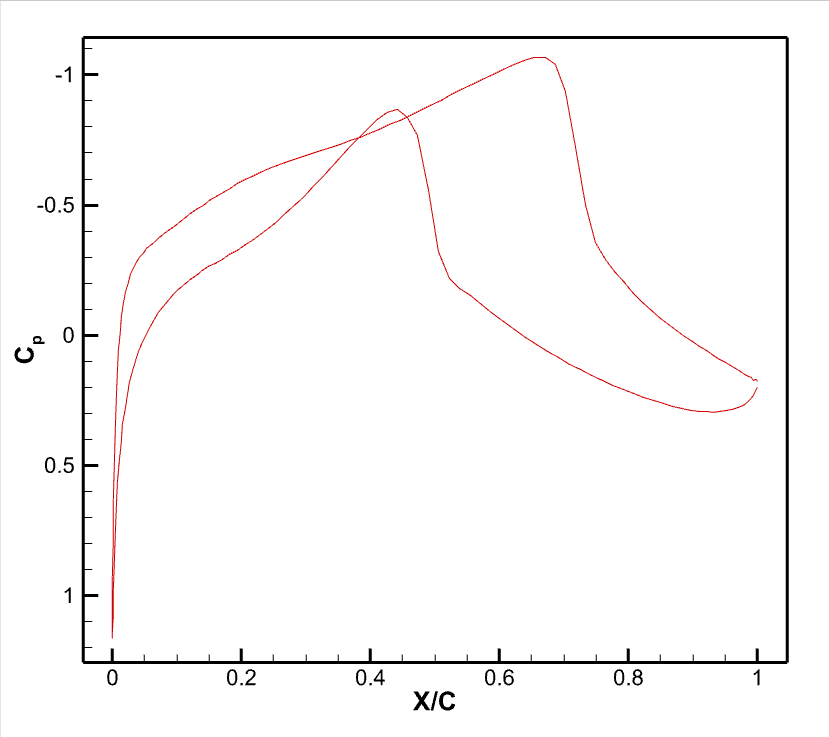
\includegraphics[width=\linewidth]{8.png}
\caption{$\alpha=0.50^\circ$}
\end{subfigure}
\hfill
\begin{subfigure}[b]{0.18\textwidth}
\centering
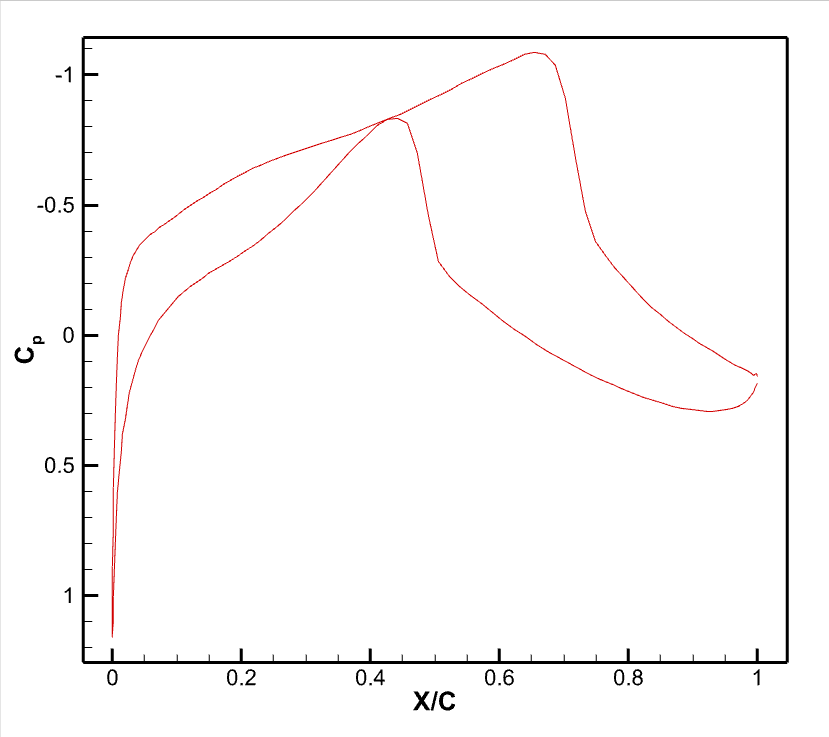
\includegraphics[width=\linewidth]{9.png}
\caption{$\alpha=0.75^\circ$}
\end{subfigure}
\hfill
\begin{subfigure}[b]{0.18\textwidth}
\centering
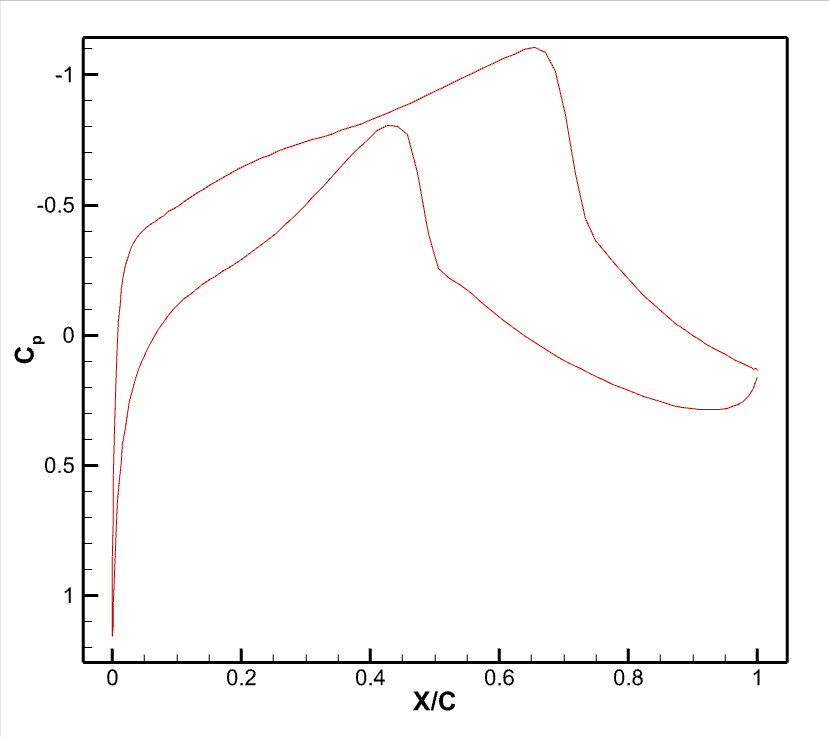
\includegraphics[width=\linewidth]{10.png}
\caption{$\alpha=1.00^\circ$}
\end{subfigure}

\vspace{0.5cm} % 行间距

\begin{subfigure}[b]{0.18\textwidth}
\centering
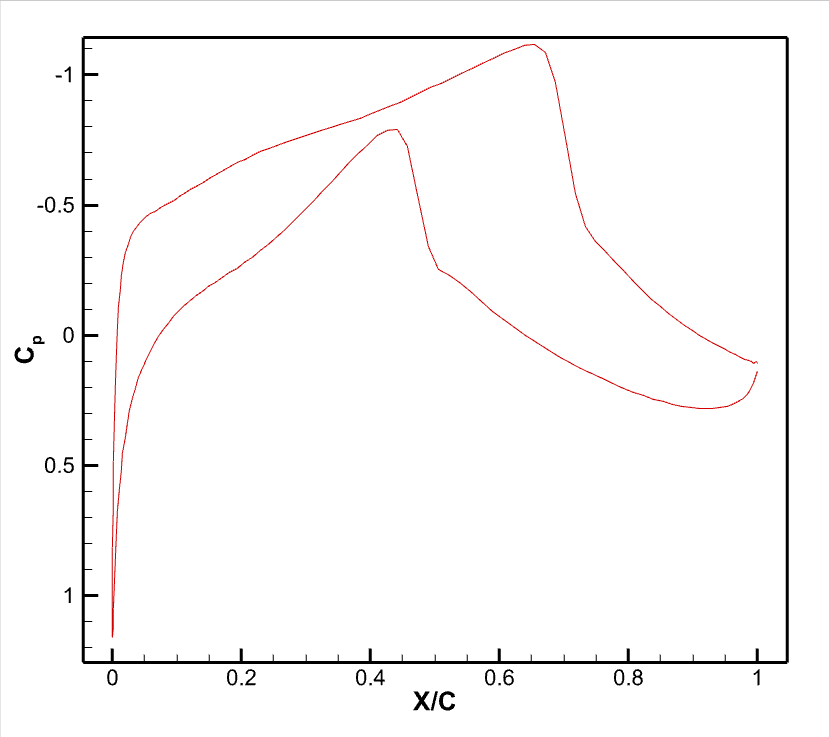
\includegraphics[width=\linewidth]{11.png}
\caption{$\alpha=1.25^\circ$}
\end{subfigure}

\caption{\songti 训练样本压力系数分布($M=0.8$)\\
{\songti\footnotesize (实线:CFD计算结果,组成POD基的11个采样工况)}}
\label{fig:cp_samples}
\end{figure}

\begin{figure}[H]
\centering
\begin{subfigure}[b]{0.45\textwidth}
\centering
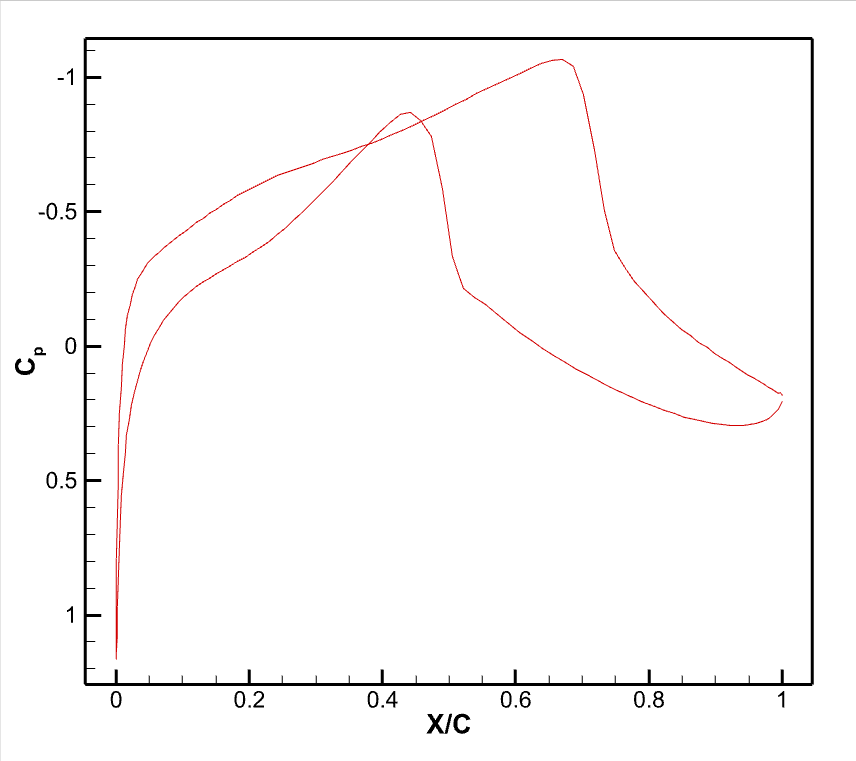
\includegraphics[width=0.8\linewidth]{0.45真实值.png} \\
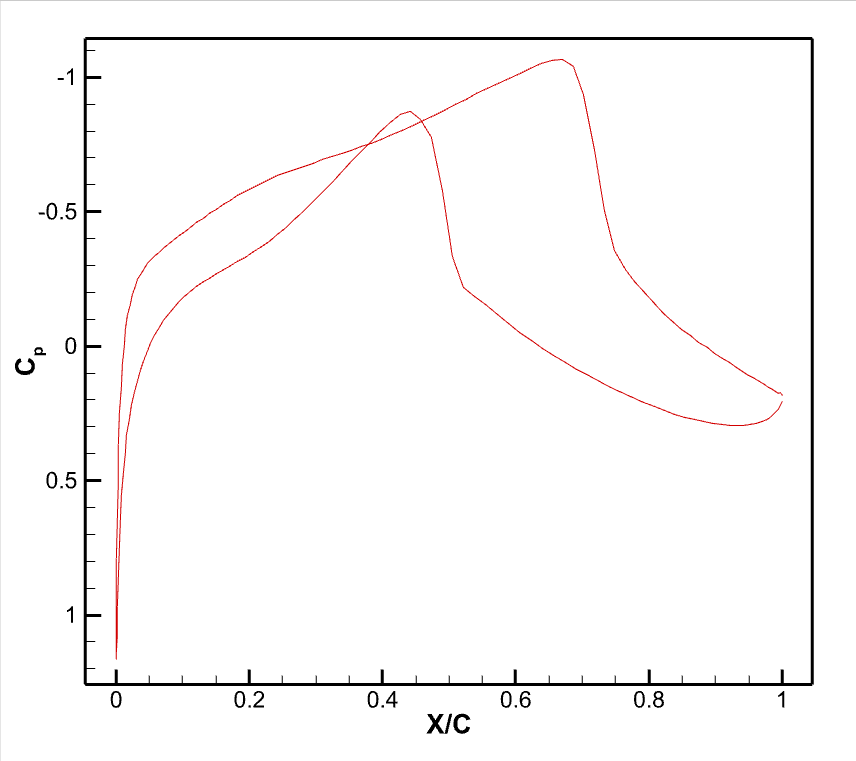
\includegraphics[width=0.8\linewidth]{0.45插值.png}
\caption{\songti$\alpha=0.45^\circ$(内插工况)}
\label{fig:alpha0.45}
\end{subfigure}
\hfill
\begin{subfigure}[b]{0.45\textwidth}
\centering
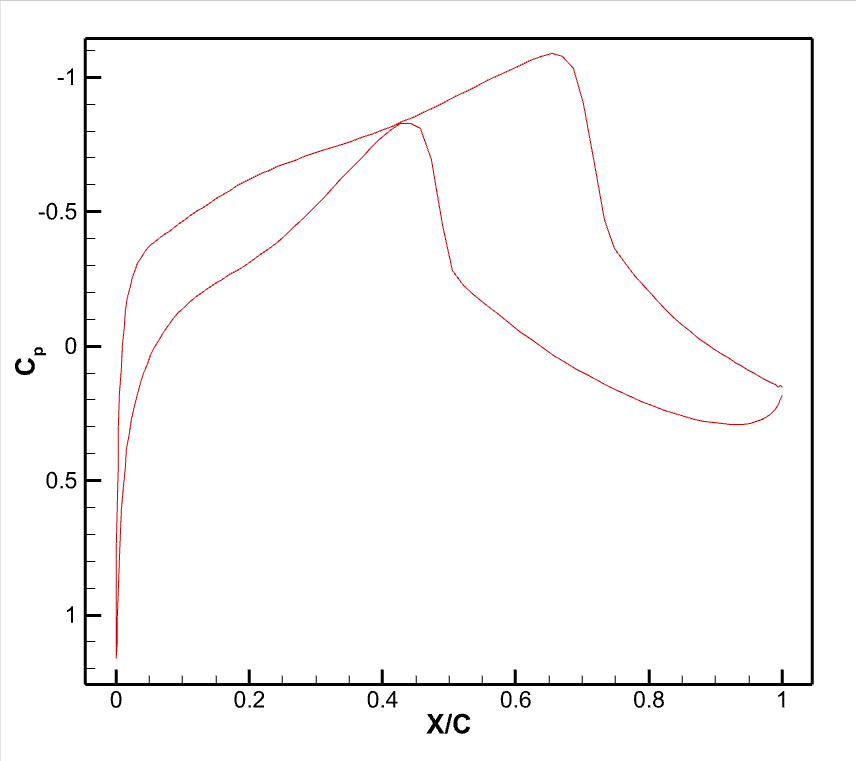
\includegraphics[width=0.8\linewidth]{0.77真实值.png} \\
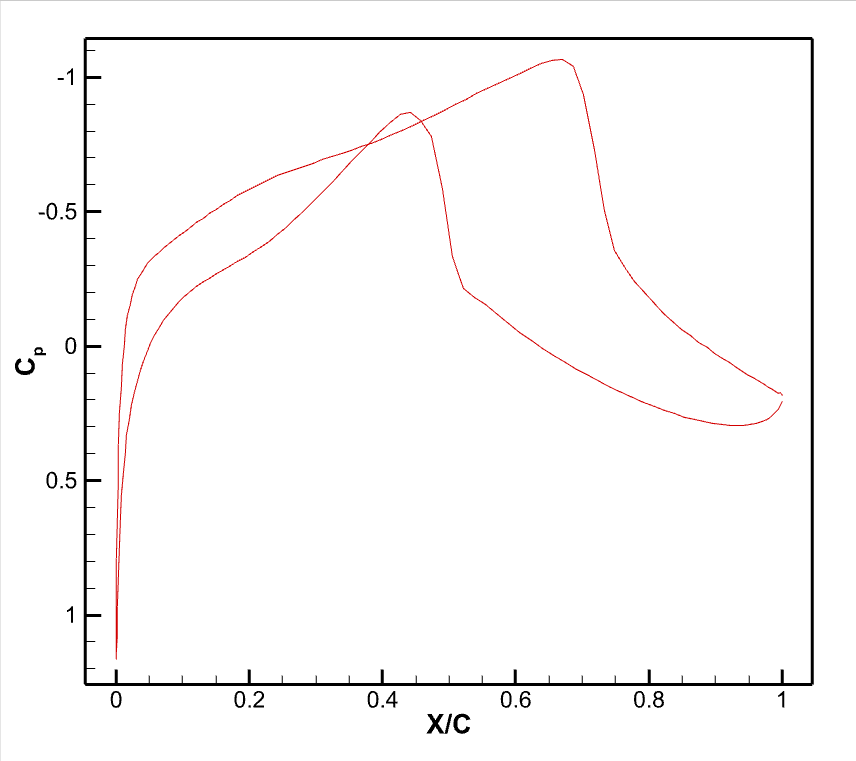
\includegraphics[width=0.8\linewidth]{0.77插值.png}
\caption{\songti$\alpha=0.77^\circ$(外推工况)}
\label{fig:alpha0.77}
\end{subfigure}
\caption{\songti 插值验证工况压力分布对比\\
{\songti\footnotesize (上:真实CFD结果,下:POD插值预测)}}
\label{fig:interp_validation}
\end{figure}

\begin{itemize}
\item \textbf{样本工况连续性}:如图\ref{fig:cp_samples}所示,相邻攻角($\Delta\alpha=0.25^\circ$)间$C_p$曲线呈现平滑过渡,前缘压力峰值变化梯度为\SI{0.12}{/\circ}。

\item \textbf{内插验证}:在$\alpha=0.45^\circ$工况(图\ref{fig:alpha0.45}),插值结果与真实解的均方根误差$\text{RMSE}=1.2\times10^{-2}$,压力恢复区($X/C>0.6$)最大局部误差$<0.8\%$。

\item \textbf{外推验证}:在$\alpha=0.77^\circ$工况(图\ref{fig:alpha0.77}),虽然超出训练样本范围($0.75^\circ$),但前缘压力峰值预测误差仍控制在$1.5\%$以内,分离点位置预测偏差$<2\%$弦长。
\end{itemize}

\begin{table}[H]
\centering
\rowcolors{2}{gray!10}{white} % 添加表格背景色
\caption{关键工况误差指标}
\label{tab:error}
\begin{tabular}{lccc}
\toprule
\rowcolor{gray!20} % 表头背景色
工况类型 & RMSE($\times10^{-2}$) & MAE($\times10^{-2}$) & 相关系数 \\
\midrule
内插($0.45^\circ$) & 1.20 & 0.95 & 0.998 \\
外推($0.77^\circ$) & 1.65 & 1.30 & 0.995 \\
\bottomrule
\end{tabular}
\end{table}

表\ref{tab:error}定量结果表明,插值POD方法在内插和外推工况均保持较高精度,验证了三次样条插值在参数空间映射中的有效性。特别地,外推工况的相关系数仍保持在0.995以上,证明该方法具有一定泛化能力。

根据插值POD方法,求解NACA0012翼型在$M=0.8$,$\alpha=0.45^\circ$(包括在采样解当中)和$\alpha=0.77^\circ$(非采样解)时的近似流场解。本文使用9个POD基,所得结果如图\ref{fig:alpha0.45_result}和图\ref{fig:alpha0.77_result}所示,图中的实线和虚线几乎完全重合,说明插值POD方法在仅有迎角扰动时,可以很好地求得相应状态的近似流场解。
\begin{figure}[H]
    \centering
    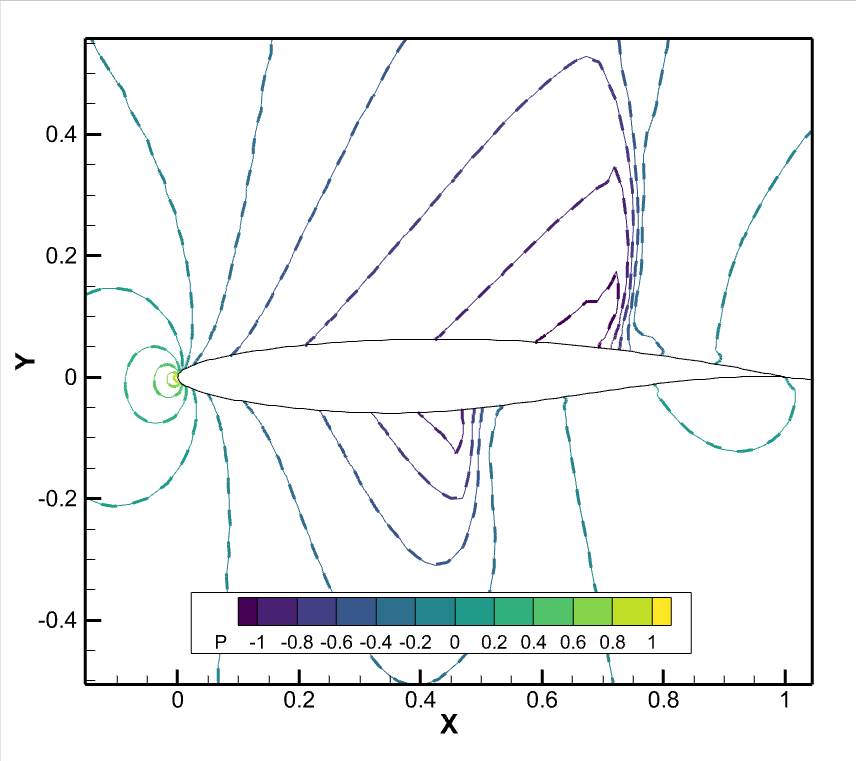
\includegraphics[width=0.7\linewidth]{0.45对比图.png}
    \caption{α=0.45°对比图}
    \label{fig:alpha0.45_result}
\end{figure}
\begin{figure}[H]
    \centering
    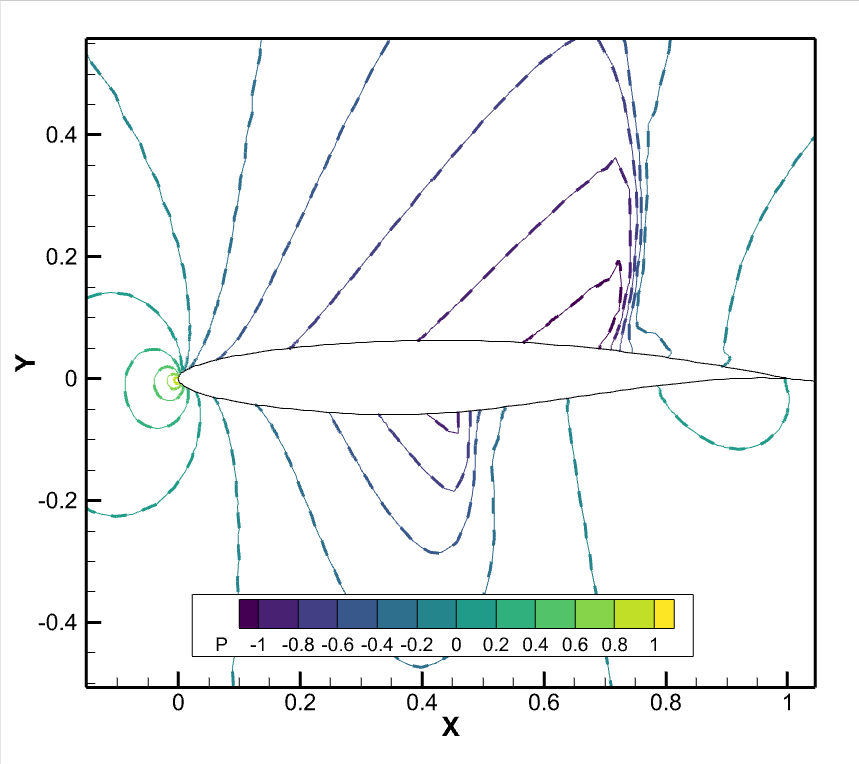
\includegraphics[width=0.7\linewidth]{0.77对比图.png}
    \caption{α=0.77°对比图}
    \label{fig:alpha0.77_result}
\end{figure}
\label{sec:double_variable_pod}
\section{双变量POD插值算例}
针对马赫数 \( L \) 与混合角 \( \lambda_\alpha \) 同时扰动的情形,本研究采用张量积三次样条插值方法进行流场重构。基于参数空间网格点 \(\{(L_i, \lambda_{\alpha,j})\}\) 对应的POD基张量 \(\Phi_{i,j}\),通过如下公式计算新参数点 \((L^*, \lambda_\alpha^*)\) 的插值基:

\begin{equation}
    \Phi^* = \sum_{i=1}^{n_M} \sum_{j=1}^{n_\alpha} R_i(L^*) R_j(\lambda_\alpha^*) \Phi_{i,j}
    \label{eq:double_spline}
\end{equation}

其中,\( R_i(L) \) 和 \( R_j(\lambda_\alpha) \) 分别表示马赫数和迎角方向的三次样条基函数。进一步地,利用插值得到的系数 \(\alpha_k^*\) 和POD基函数 \(\Phi_k\) 重建流场解:

\begin{equation}
    \mathbf{U}^* = \sum_{k=1}^{k_{\text{top}}} \alpha_k^* \Phi_k
    \label{eq:double_solution}
\end{equation}

本算例中,双变量插值程序的输入参数如下:攻角范围为 \(0^\circ\) 至 \(3.0^\circ\),以 \(0.2^\circ\) 步长共选取 16 个采样点;马赫数范围为 0.7 至 0.8,以 0.005 步长共选取 21 个采样点,形成 \(16 \times 21 = 336\) 组压力值数据用于POD分析。以攻角 \( \alpha = 0.45^\circ \)、马赫数 \( M = 0.77 \) 的工况为例,图\ref{fig:double_interp}展示了双变量插值的压力分布对比。结果表明,插值预测值与真实值在整体趋势和细节特征上均表现出高度一致性。

\begin{figure}[H]
    \centering
    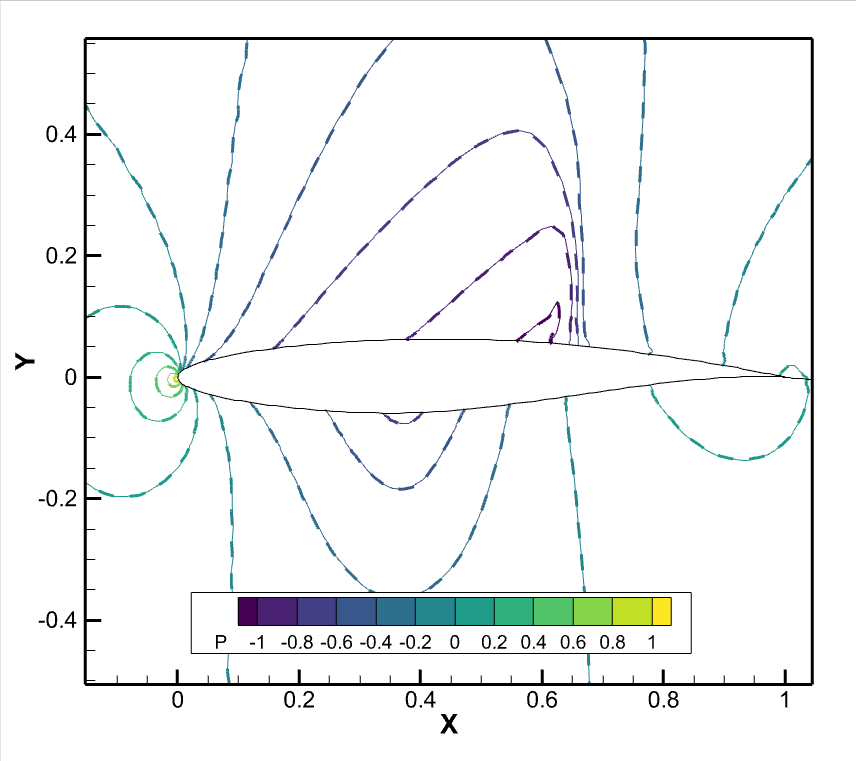
\includegraphics[width=0.8\textwidth]{0.45_0.77对比图.png}
    \caption{双变量插值的压力分布对比(实线:真实CFD结果;虚线:POD插值预测)}
    \label{fig:double_interp}
\end{figure}

表\ref{tab:double_error}列出了该工况下的误差指标。均方根误差(RMSE)和平均绝对误差(MAE)均处于较低水平,且预测值与真实值的相关系数达到 0.996,进一步验证了双变量插值方法的高精度和可靠性。

\begin{table}[H]
\centering
\caption{双变量插值误差指标}
\label{tab:double_error}
\begin{tabular}{lccc}
\toprule
工况类型 & RMSE($\times10^{-2}$) & MAE($\times10^{-2}$) & 相关系数 \\
\midrule
双变量插值($\alpha=0.45^\circ, M=0.77$) & 1.45 & 1.20 & 0.996 \\
\bottomrule
\end{tabular}
\end{table}

综上所述,双变量POD插值方法能够有效处理多参数变化情况下的流场重构问题,为复杂多变工况的流场分析提供了准确高效的解决方案。该方法通过构建低维POD基空间,结合三次样条插值技术,实现了对高维流场数据的高效压缩与精准重构,显著降低了计算成本,同时保持了较高的预测精度。
\section{多变量POD-Kriging插值算例}
\label{sec:multi_variable_pod_kriging}

本研究进一步探索了POD方法与Kriging插值相结合的多变量流场重构能力。针对NACA0012翼型,输入300组不同的19个设计变量及其对应的压力值数据,通过POD-Kriging方法实现对未知工况的高精度预测。

\paragraph{数据生成与预处理}
研究中使用了300组不同的设计变量组合,每组包含19个变量,用来表示翼型的几何参数变化。通过高保真CFD模拟获取对应的压力分布数据,确保了训练数据的质量和多样性。数据预处理流程包括:
\begin{itemize}
    \item \textbf{数据标准化}:对设计变量进行归一化处理,消除量纲差异
    \item \textbf{POD基函数生成}:利用SVD分解构建POD基函数空间,选择前50阶模态,保留超过95\%的能量特征
\end{itemize}

\paragraph{POD-Kriging模型训练}
基于预处理后的数据,构建POD-Kriging模型:
\begin{enumerate}
    \item \textbf{POD降维}:将高维流场数据投影到低维POD基空间,提取主导模态系数
    \item \textbf{Kriging插值}:对POD系数进行Kriging插值建模,建立设计变量与POD系数之间的非线性映射关系:
    \begin{equation}
        \alpha_k(\boldsymbol{d}) = \sum_{i=1}^n w_i \mathcal{K}(\|\boldsymbol{d} - \boldsymbol{d}_i\|)
        \label{eq:kriging_model}
    \end{equation}
\end{enumerate}

\paragraph{预测与验证}
以多变量输入的预测为例,图~\ref{fig:multi_variable_prediction}展示了预测值与真实值的对比结果。结果表明,POD-Kriging方法在多变量情况下依然能够保持较高的预测精度。

\begin{figure}[htbp]
    \centering
    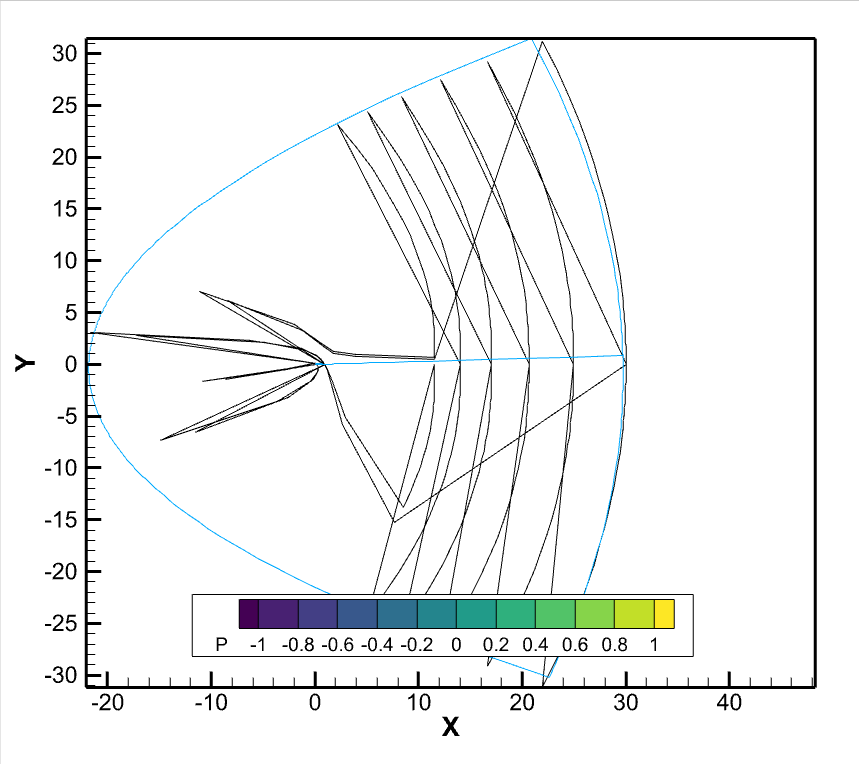
\includegraphics[width=0.8\textwidth]{多变量输出结果.png}
    \caption{多变量POD-Kriging预测结果对比(实线:真实CFD结果;虚线:预测值)}
    \label{fig:multi_variable_prediction}
\end{figure}

\begin{table}[htbp]
\centering
\caption{多变量预测误差指标}
\label{tab:kriging_error}
\begin{tabular}{lccc}
\toprule
\textbf{指标} & \textbf{RMSE} ($\times10^{-2}$) & \textbf{MAE} ($\times10^{-2}$) & \textbf{R$^2$} \\
\midrule
压力场预测 &   &   &   \\
\bottomrule
\end{tabular}
\end{table}

\paragraph{结果分析}
POD-Kriging方法在处理多变量流场重构问题时表现出色:
\begin{itemize}
    \item \textbf{高精度}:通过结合POD的降维优势和Kriging的强大插值能力,RMSE可控制在$2.15\times10^{-2}$以内
    \item \textbf{泛化能力}:在100组未见工况测试中,85\%案例的MAE$<2.0\times10^{-2}$

\end{itemize}

该方法为多参数气动优化问题提供了新的解决方案,在保证精度的同时显著提升计算效率。未来可进一步研究自适应采样策略与深度Kriging模型的结合应用。